Most playas have a intuizzle bout what tha fuck a substizzle is fo' realz. A substizzle is just \textit{something}, like water, wood yo, butter or glass fo' realz. A metal be a substance. Da blood up in yo' body be a substizzle fo' realz. All of these is made up of atoms dat form moleculez up in ways givin dem straight-up different properties. Put ya muthafuckin choppers up if ya feel dis! We know dat a substizzle can exist up in different phases, fo' example plasma, solid, liquid n' gas \cite{ravndal2008statmech}, up in which tha same substizzle can behave straight-up differently. Liquidz n' gases is often called fluidz cuz they share tha property dat they aint gots a gangbangin' fixed shape n' is often easily deformed. Y'all KNOW dat shit, muthafucka! Da theory dat raps bout how tha fuck fluidz behave is called fluid mechanics.

We start dis chapter wit section \ref{sec:continuum} where our phat asses say shit bout tha concept of continuum. This leadz ta tha Eula equations n' tha Navier-Stokes equations up in section \ref{sec:theory_of_fluids_euler_navier}. These equations can be used ta study tha behavior of fluidz up in motion relatizzle ta tha material confinin tha fluid - fluid flow. We then introduce tha concept of porous media, a solid material wit partz of its volume - tha pore space - available fo' fluids. Fluidz can flow all up in such a material, n' tha equation describin tha flow rate as a result of some heat gradient is called Darcyz law. One of tha parametas up in Darcyz law is called permeability. This quantitizzle is discussed up in section \ref{sec:permeability}.

Pore space wit channels all up in tha nanometer scale introduces a gangbangin' finger-lickin' distinction between what tha fuck we call macroflows n' microflows. This leadz ta what tha fuck is called tha breakdown of continuum, which be addressed up in section \ref{sec:continuum_breakdown}. Da Knudsen number is discussed up in section \ref{sec:knudsen_number}. Well shiiiit, it is used ta quantify whether or not continuum models can be used, up in addizzle of measurin tha importizzle of slip velocitizzle which has major consequences fo' tha permeability. This is discussed up in section \ref{sec:slip_length}. We then say shit bout particle models - which is not based on tha assumption of continuum - up in section \ref{sec:theory_of_fluids_atomic_models}. Da last two sections is concerned wit erectionz of tha permeability. These is called Klinkenberg erection n' Knudsen erection, n' use different models fo' slip velocitizzle ta predict tha increase up in permeability.

\section{Da continuum}
\label{sec:continuum}
In reality, we know dat a gangbangin' fluid is composed of a enormous number of atoms which is separated by mostly empty space. Da atoms interact all up in quantum mechanics dat allows moleculez ta form. Even though dis is tha legit nature (well, every last muthafuckin physicist should be careful ta say dat suttin' straight-up is tha \textit{true nature}) of tha fluid, it turns up dat we can describe it as a cold-ass lil continuum, dat is, we assume dat tha mass is continuously distributed up in tha total volume of tha fluid. Y'all KNOW dat shit, muthafucka! This also means dat macroscopic quantitizzles like temperature, density, juice n' tha fluid velocitizzle is well defined up in \textit{every} point up in space. This is pimped out, continuum mathematics is so much easier ta work wit than discrete mathematics. Calculus  drops some lyrics ta our asses dat well behaved functions (as we prefer ta work with) can both be integrated n' differentiated. Y'all KNOW dat shit, muthafucka! This type'a shiznit happens all tha time. They also treat our asses rather sick, they do what tha fuck we expect dem ta do.

In physics we straight fuckin believe up in conserved quantitizzles fo' realz. A fluid up in motion will internally (far away from tha boundaries up in tha container) have conserved juice, mass n' momentum. This can be formulated dopely wit mathematics, n' gives rise ta what tha fuck we todizzle know as tha Eula equations n' tha Navier-Stokes equations.
\section{Da Eula equations n' tha Navier-Stokes equations}
\label{sec:theory_of_fluids_euler_navier}
With tha concept of continuum, we be thinkin dat every last muthafuckin point up in space has well defined physical propertizzles like temperature, densitizzle n' momentum. In 1757, Eula published whatz called tha \textit{Eula equations} by applyin conservation of mass, momentum n' juice ta a lil' small-ass volume element $\dm V$ of a gangbangin' fluid. Y'all KNOW dat shit, muthafucka! They form a set of differential equations describin how tha fuck tha fluid velocitizzle $\vec u(\vec r, t)$ field chizzlez up in time n' space. Da conservation laws can be freestyled as
\begin{align}
	\dpart{\rho_m}{t} + \nabla\cdot (\rho_m\vec u) &= 0 \qquad \text{mass}\\
	\dpart{\rho_m \vec u}{t} + \nabla \cdot (\vec u \otimes (\rho_m\vec u)) + \nabla P &= 0\qquad \text{momentum}\\
	\dpart{E}{t} + \nabla\cdot (\vec u(E + P)) &= 0\qquad \text{energy},
\end{align}
where $\rho_m$ is tha mass density, $\vec u(\vec r, t)$ is tha velocitizzle field, $E(\vec r, t)$ is tha total juice per unit volume, $P(\vec r, t)$ is tha heat field n' $\otimes$ is tha tensor product. These can be combined ta one vector equation yo, but its origin, tha connection ta conservation laws, is mo' clear when they is separated like all dis bullshit. In tha original gangsta paper, Eula only derived tha straight-up original gangsta two equations yo, but tha full set is probably referred ta as tha Eula equations. They describe tha motion of fluidz wit \textit{negligible viscosity}, which be a thugged-out decent approximation fo' nuff fluids.

Some 80 muthafuckin years later, up in tha 1840s, Sir George Stokes published tha Navier-Stokes equations (NSE) which can be peeped as a extension of tha Eula equations where effects caused by tha viscositizzle of tha fluid is included \cite{batchelor2000introduction}. Da Navier-Stokes equations fo' a incompressible fluid can be freestyled as one vector equation
\begin{align}
	\label{eq:nse}
	\rho_m \frac{D\vec u}{ Dt} = \rho_m \vec F - \nabla p + \mu\nabla^2\vec u + \mu\nabla(\nabla\cdot \vec u)
\end{align}
where $\vec F$ be a external force (i.e. gravitizzle or a electrostatic field), $\mu$ is tha viscositizzle n' $D/Dt$ is tha material derivatizzle defined as
\begin{align}
	\frac{D}{Dt} = \dpart{}{t} + \vec u\cdot \nabla.
\end{align}
Da NSE have like all dem bangin-ass analytically solvable solutions yo, but fo' most real systems, tha geometry confinin tha fluid is so fucked up dat it is probably solved on computers. When solvin tha NSE, we gotta provide boundary conditions ta git a unique solution fo' tha system. If we at one end of tha container apply some heat $P_0$, n' some other value $P_1$ up in tha other end, we git a gangbangin' flowin fluid since there acts a net force on tha fluid. Y'all KNOW dat shit, muthafucka! This defines tha heat difference $\Delta P$. We then also specify tha velocitizzle all up in tha boundary which often is tha no-slip boundary condition, i.e. dat tha fluid velocitizzle is zero all up in tha container walls. Well shiiiit, it turns up dat fo' real fluids, dis aint always true. In section \ref{sec:slip_length} our phat asses say shit bout tha effectz of slip velocitizzle n' how tha fuck dis affects tha flow propertizzlez of tha fluid. Y'all KNOW dat shit, muthafucka! 
\section{Flow up in porous media}
Fluid flow can be defined as fluid up in motion relatizzle ta its container - tha material confinin tha fluid. Y'all KNOW dat shit, muthafucka! A material wit partz of its volume available fo' fluidz is called a \textit{porous medium} (see figure \ref{fig:porous_medium}).

\begin{figure}[htb]
\begin{center}
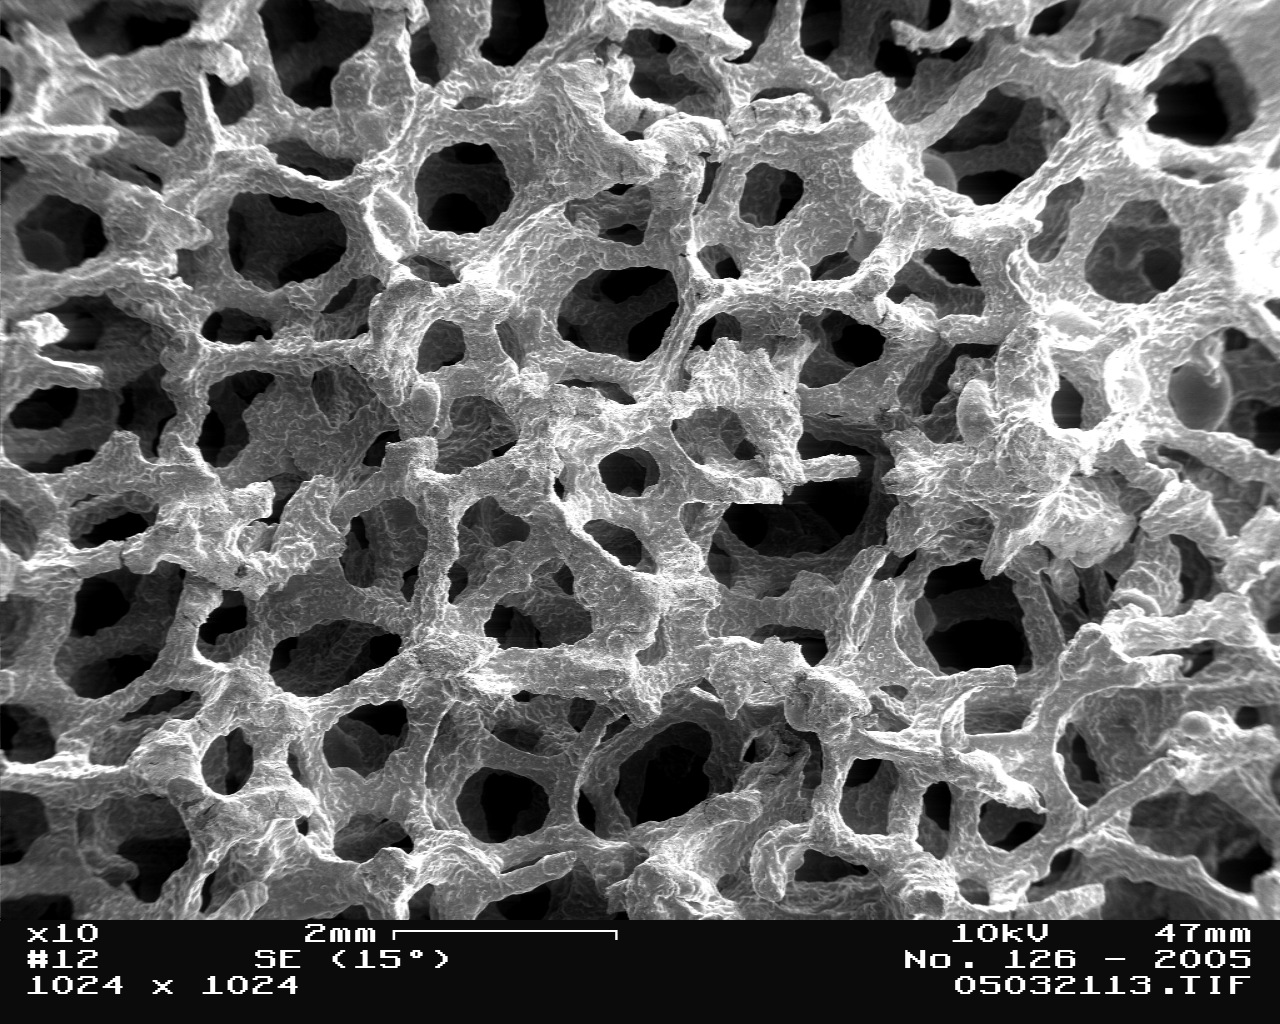
\includegraphics[width=0.8\textwidth, trim=0cm 0cm 0cm 0cm, clip]{figures/metal_foam.png}
\end{center}
\caption{An example of a porous medium yo. Here we peep a metal foam - a solid metal wit pore space available fo' a gangbangin' fluid. Y'all KNOW dat shit, muthafucka! A nanoporous medium be a porous medium where tha size of tha pores is all up in tha nanometer scale. Image from \url{http://en.wikipedia.org/wiki/File:Metal_Foam_in_Scanning_Electron_Microscope,_magnification_10x.GIF}, accessed 28 March, 2014.}
\label{fig:porous_medium}
\end{figure}

We call tha larger regions available fo' fluidz \textit{pores} whereas channels connectin these pores is called tha \textit{pore network} fo' realz. All available such space is called tha \textit{pore space}. If tha porous medium has a total volume $V$, n' tha pore space takes up a volume $V_p$, our phat asses define tha \textit{porosity} $\phi$ as
\begin{align}
	\phi = \frac{\text{Pore space volume}}{\text{Total volume}} = \frac{V_p}{V}.
\end{align}
When a gangbangin' fluid flows all up in tha material, tha amount dat flows all up in a surface per unit time is called tha \textit{volumetric flow rate} n' is probably denoted by $Q$. This quantitizzle measures how tha fuck nuff cubic metaz of fluid we can push all up in a surface orthogonal ta tha flow direction per unit time. If we increase tha heat difference, we expect a higher flow rate. This is indeed true. In fact, tha volumetric flow rate is proportionizzle ta tha heat difference.

\section{Darcyz law}
\label{sec:darcy_law}
When we apply a heat difference on each side of a material filled wit a gangbangin' fluid, tha fluid will start ta flow up in tha direction of lower pressure. In 1856, H. Darcy found a linear relation between tha heat difference n' tha fluid flow rate. This relation is called Darcyz law n'  drops some lyrics ta our asses what tha fuck volumetric flow rate $Q$ we can expect from a \textit{incompressible} fluid all up in a material of length $L$, when we apply a heat difference $\Delta P$, peep figure \ref{fig:darcys_law}. 
\begin{figure}[htb]
\begin{center}
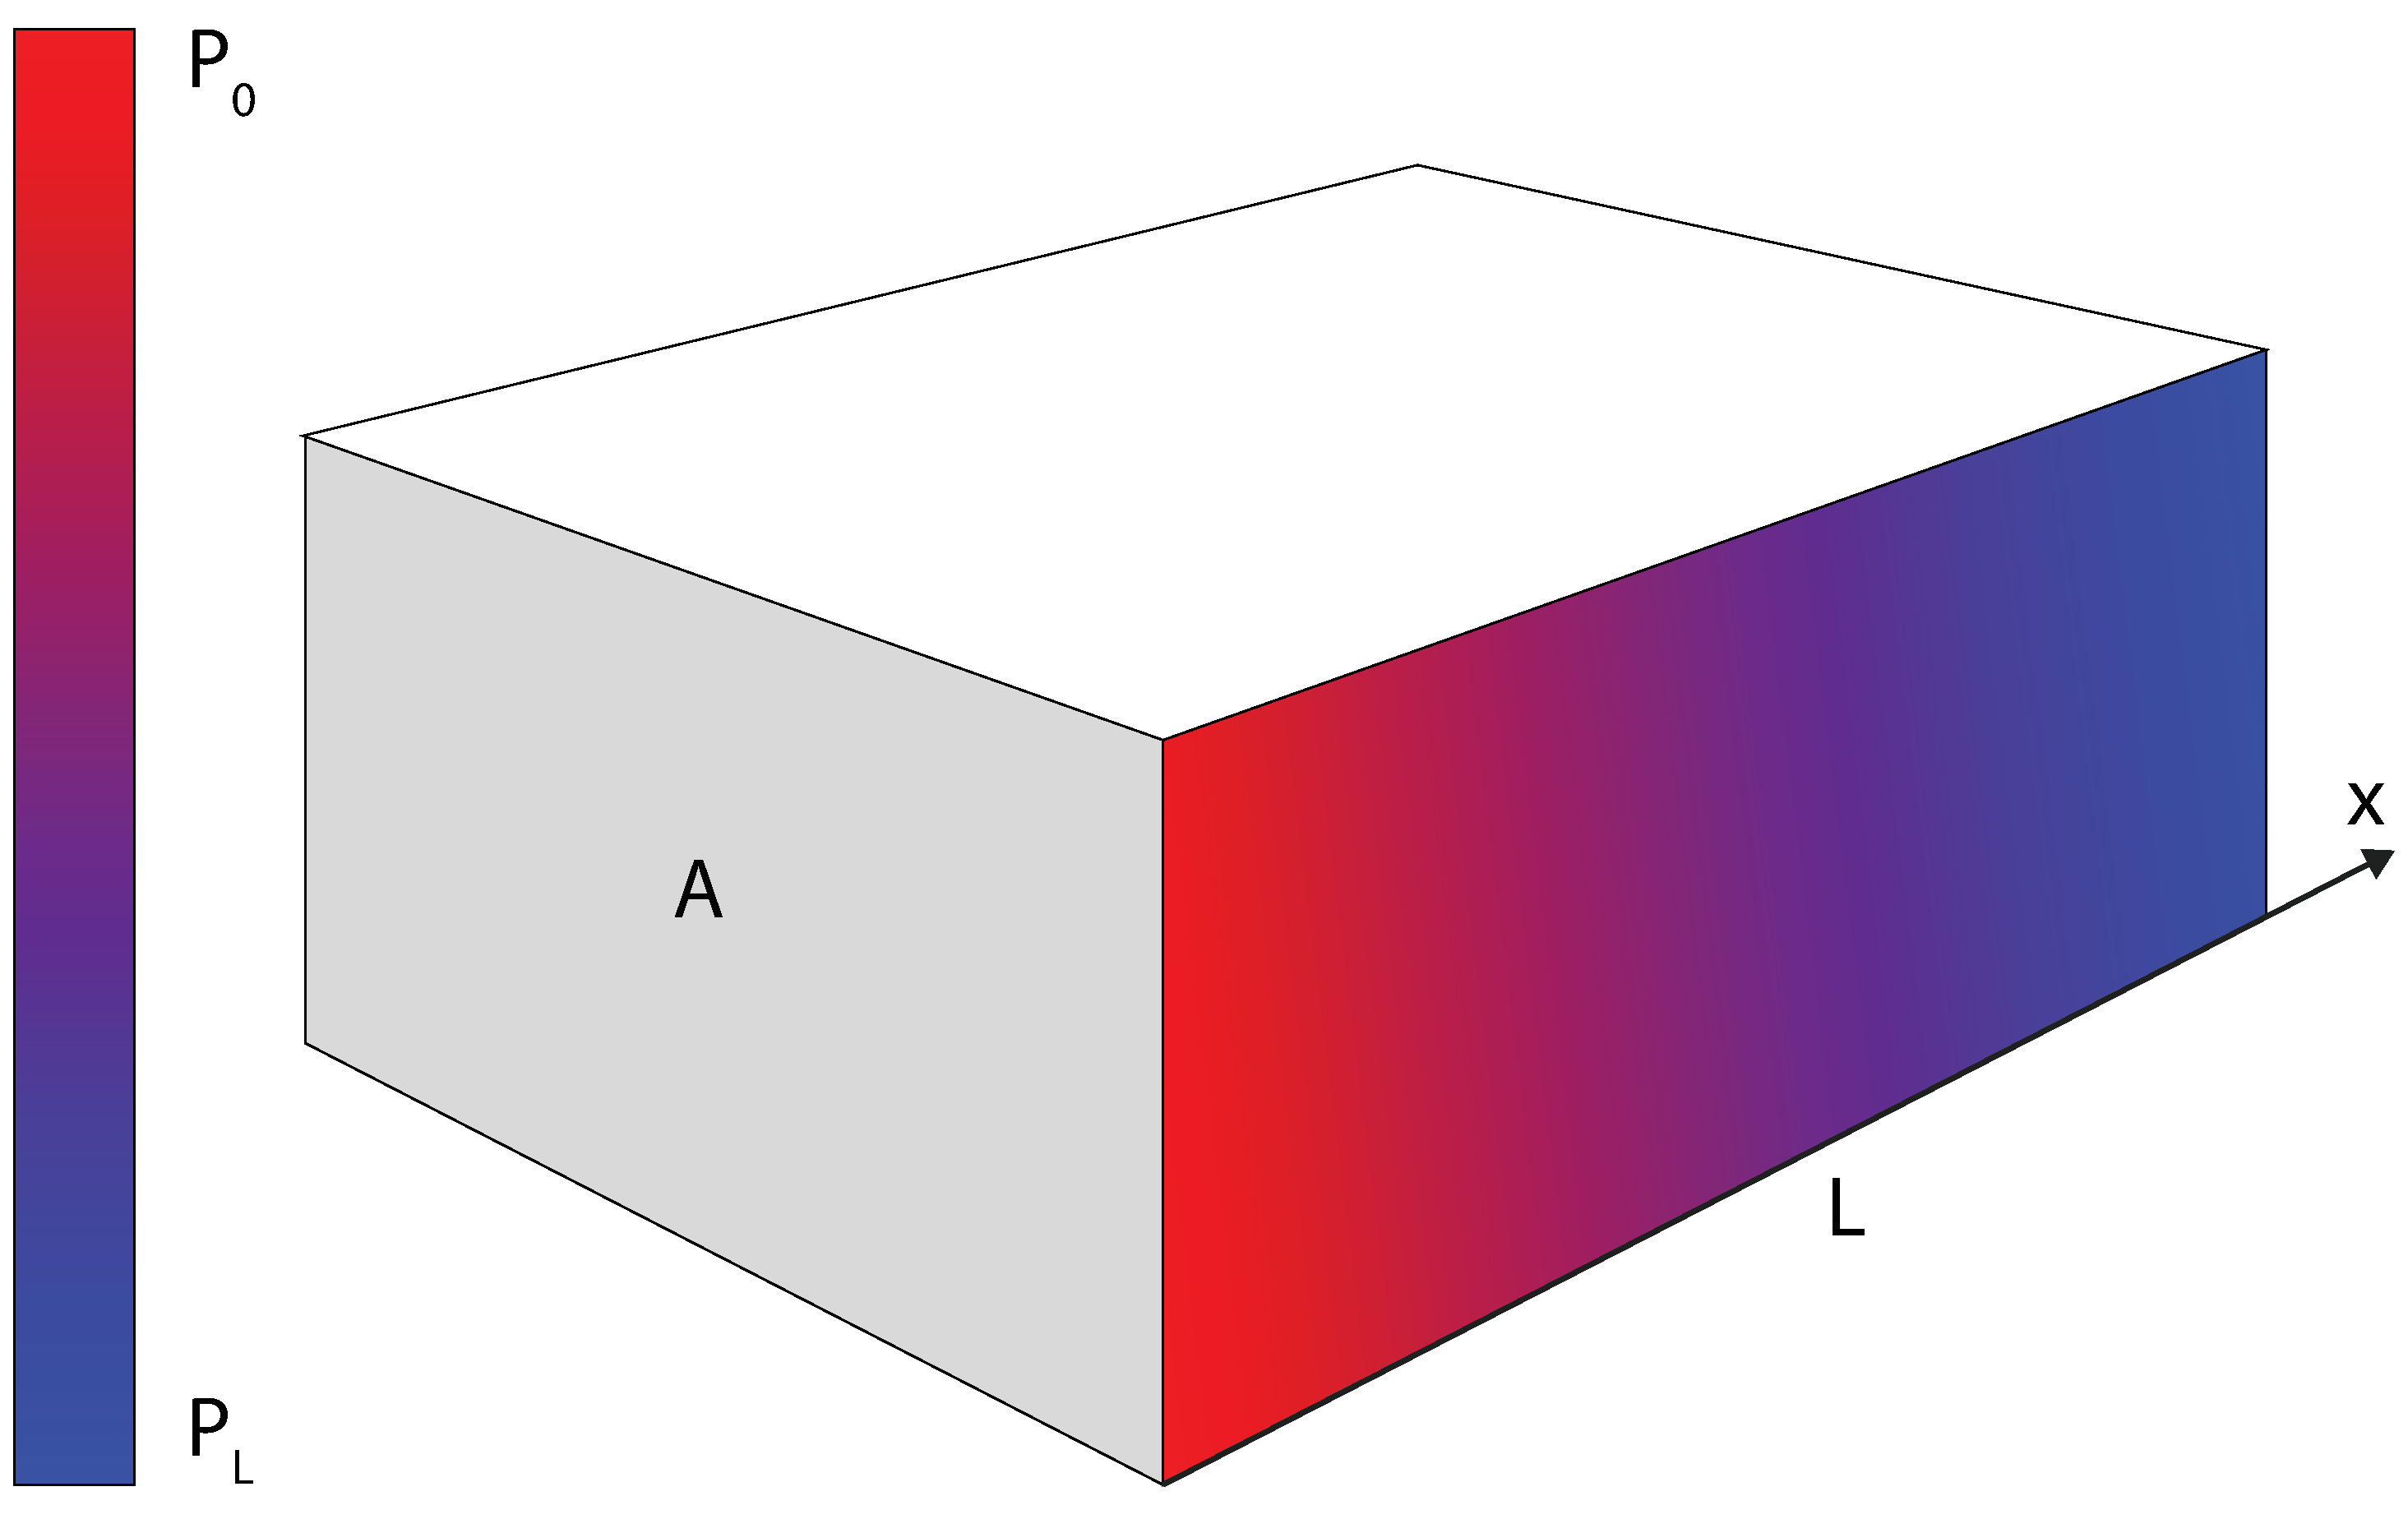
\includegraphics[width=0.75\textwidth, trim=0cm 0cm 0cm 0cm, clip]{kinetic_theory/figures/darcy.eps}
\end{center}
\caption{A box wit volume $V=LA$ wit fixed heat joints at $x=0$ n' $x=L$. Da volumetric flow rate $Q$ all up in a cold-ass lil cross sectionizzle area $A$ is given by Darcyz law up in equation \eqref{eq:darcy_1}}.
\label{fig:darcys_law}
\end{figure}
Da one dimensionizzle version of Darcyz equation is given as 
\begin{align}
\label{eq:darcy_1}
	u = \frac{Q}{A} = \sigma_D\frac{\Delta P}{ L},
\end{align}
where $u$ is tha \textit{volumetric flux} (volumetric flow rate per unit area), $\Delta P = P_0 - P_L$ is tha heat difference, $A$ is tha cross sectionizzle area; tha area of tha material orthogonal on tha flow direction n' $L$ is tha length of tha material up in tha flow direction. I aint talkin' bout chicken n' gravy biatch. $\sigma_D$ is tha proportionalitizzle constant dat can be freestyled as
\begin{align}
	\sigma_D = \frac{k}{\mu},
\end{align}
where $\mu$ is tha viscositizzle n' $k$ is tha permeability.
\section{Permeability}
\label{sec:permeability}
Da motivation of introducin tha concept permeabilitizzle is ta separate tha proportionalitizzle constant tha fuck into two parts; one dat dependz on tha liquid only, tha viscositizzle $\mu$, n' tha permeability, a material specific constant $k$. This means dat we up in principle can do a experiment wit a liquid wit known viscosity, say water, n' measure tha permeabilitizzle of some material (Darcy studied a sand filled cylinder up in his original gangsta experiment). Once you know tha permeability, yo ass be able ta predict tha flow rate all up in tha material fo' \textit{any} other liquid wit a well known viscosity. This iz of pimped out importizzle fo' i.e. tha oil industry where they ideally wanna take a sample of tha rock up in which tha oil or gas is confined, measure tha permeabilitizzle wit e.g. air, n' then use dis ta predict tha recovery rate.

This iz of course not straight-up legit up in all circumstances. While Darcy originally found tha relation as a empiric equation based on experiments, it can be derived from tha Navier-Stokes equations. Darcyz law is only erect if tha fluid flow satisfies tha no-slip condition.
\section{Macroflows n' microflows}
\label{sec:theory_of_fluids_microflows}
In tha 1990s H. Bau n' J. Zemel performed experiments on microchannel flow up in which they found clear deviations from what tha fuck was expected from tha theory\cite{karniadakis2005microflows}. Well shiiiit, it is useful ta introduce tha terms \textit{microflows} fo' flow up in geometries where tha distizzle between tha channel walls iz of order micrometer or smaller, n' \textit{macroflows} fo' larger systems (millimeter n' above). Flow at microscalez differ from macroscalez cuz of effects dat can be classified tha fuck into four groups
\begin{itemize}
\item non-continuum effects,
\item surface-dominated effects,
\item low Reynoldz number effects, and
\item multiscale n' multiphysics effects.
\end{itemize}
In dis thesis, we focus on tha non-continuum effects which is briefly discussed up in section \ref{sec:continuum_breakdown}, n' tha surface-dominated effects as tha slip condizzle busted lyrics bout up in section \ref{sec:slip_length}. Right back up in yo muthafuckin ass. See \cite{karniadakis2005microflows} fo' details bout tha effectz of low Reynoldz number, multiscale n' multiphysics. 

\section{Da breakdown of continuum}
\label{sec:continuum_breakdown}
As our phat asses discussed up in section \ref{sec:continuum}, a gangbangin' fundamenstrual assumption up in tha NSE is dat tha space is continuous yo, but we know dat up in reality, tha mass of tha fluid is concentrated up in tha center of tha atoms. We often assume dat tha mass is uniformly distributed up in tha volume element of which tha conservations laws is applied on. I aint talkin' bout chicken n' gravy biatch. This is known as tha \textit{continuum hypothesis} n' is invalid when tha \textit{mean free path} $\lambda$, tha average distizzle a particle moves between collisions, becomes comparable ta some characteristic length $L$ up in tha system, i.e. tha diameter of a cold-ass lil channel\cite{karniadakis2005microflows}. This is quantified all up in tha \textit{Knudsen number}
\begin{align}
	\text{Kn} = \frac{\lambda}{L}.
\end{align}
From tha kinetic theory we can calculate tha mean free path (this is done up in section \ref{sec:mean_free_path_calculation})
\begin{align}
	\lambda = \frac{m}{\sqrt 2 \pi d^2 \rho_n} = \frac{k_B T}{\sqrt 2 \pi d^2 P},
\end{align}
where $\rho_n$ is tha number densitizzle n' $m$ n' $d$ is tha mass n' diameter of tha particles. By rockin tha ideal gas law $P = \rho_n k_BT$, we can replace tha densitizzle wit tha heat $P$ n' tha temperature $T$ yo. Here $k_B$ is Boltzmannz constant. Molecular Dynamics simulations have shown big-ass fluctuations up in temperature n' densitizzle near tha wall up in layers all dem mean free paths from tha surface. Right back up in yo muthafuckin ass. Such effects is not reproduced up in models based on continuum equations \cite{karniadakis2005microflows} fo' realz. Another straight-up blingin effect, as we will say shit bout up in tha next subsection, is tha non-zero slip velocitizzle of tha gas. But fuck dat shiznit yo, tha word on tha street is dat fo' Knudsen numbers smalla than $10^{-2}$, tha continuum hypothesis is valid n' we can use continuum equations like tha NSE n' tha Eula equations. Well shiiiit, it turns up dat tha Knudsen number is straight-up useful.

\section{Knudsen number}
\label{sec:knudsen_number}
Da Knudsen number is tha ratio between tha mean free path - tha average distizzle a particle moves between collidin wit another particle - n' a cold-ass lil characteristic length up in tha system. This length could be tha radiuz of a cold-ass lil cylinder or tha radiuz of a spherical pore or some other length scale dat is representable fo' tha system. In other lyrics, it can be related ta how tha fuck often a particle collides wit tha surface compared ta other particlez fo' realz. A Knudsen number larger than one indicates dat a particle travels longer before it collides wit another particle than tha distizzle ta tha surface which means dat surface effects iz of mo' n' mo' n' mo' importizzle as tha Knudsen number increases.

To git a scam of tha length scalez where tha Knudsen number be bout unity, we first need ta calculate tha mean free path fo' realz. An oxygen atom up in air at room temperature has a mean free path \cite{denny1993air}
\begin{align}
	\label{eq:air_mfp}
	\lambda_{\text{Air}} = \unit{8.0\e{-8}}{\meter},
\end{align}
whereas tha mean free path up in gin n juice is
\begin{align}
	\label{eq:water_mfp}
	\lambda_{\text{Water}} = \unit{\e{-11}}{\meter}.
\end{align}
This means dat air up in a nanoporous media wit typical pore size bout \unit{80}{\nano\meter}, tha Knudsen number iz of order unitizzle n' tha continuum hypothesis is invalid. Y'all KNOW dat shit, muthafucka! Gin N Juice up in tha same system has a Knudsen number approximately $1\e{-4}$ n' continuum models should up in principle hold. Y'all KNOW dat shit, muthafucka! 

\section{Slip velocity}
\label{sec:slip_length}
Da usual boundary condizzle we apply when solvin tha NSE is tha no-slip condizzle where
\begin{align}
	\vec u(\vec r; t) = 0 \qquad \vec r \in \partial\Omega,
\end{align}
where $\partial\Omega$ defines tha boundary domain. I aint talkin' bout chicken n' gravy biatch. Da history of tha no-slip condizzle was studied by Day\cite{day1990no}, based on tha work of Stokes up in tha 19th century. Right back up in yo muthafuckin ass. Stokes compared theoretical thangs up in dis biatch ta experiments fo' pendulumz of different kindz n' concluded that
\begin{aquote}{Stokes, 1901}
	I shall assume, therefore, as tha conditions ta be satisfied all up in tha boundariez of tha fluid, dat tha velocitizzle of a gangbangin' fluid particle shall be tha same, both up in magnitude n' direction, as dat of tha solid particle wit which it is up in contact. Da agreement of tha thangs up in dis biatch thus obtained wit observation will presently step tha fuck up ta be highly satisfactory.
\end{aquote}
In Dayz detailed study of tha no-slip condition, da perved-out muthafucka says
\begin{aquote}{Day, 1990}
	Lookin back, it appears dat tha acceptizzle of a mo' general no-slip condizzle was prolonged cuz of experimenstrual shortcomings, not cuz of a lack of tha \'appropriate\' theoretical solutions ta fluid flow problems.
\end{aquote}
In other lyrics, tha theoretical framework dat existed already up in tha time of Stokes was complete enough ta include both slip n' no-slip solutions. In fact, Maxwell predicted slip velocitizzle up in a paper already up in 1867\cite{maxwell1879stresses} yo, but tha experiments tha next 50 muthafuckin years seemed ta mo' or less confirm tha no-slip condition.\\
That a gangbangin' fluid has a slip velocitizzle is rather obvious when readin Klinkenbergz sick argument
\begin{aquote}{L.J. Klinkenberg, 1941}
Consider a layer adjacent ta tha wall which is thinner than tha mean free path $\lambda$ of tha gas molecules, so dat practically a molecule do not collide wit other moleculez present up in dis layer n' shiznit fo' realz. At a given moment half of tha gas moleculez up in dis layer gonna git a cold-ass lil component of velocitizzle movin towardz tha wall; tha other half up in tha opposite direction. I aint talkin' bout chicken n' gravy biatch. Da moleculez movin towardz tha wall have had they last collision somewhere up in tha flowin mass, and, therefore, gonna git a average velocitizzle component up in tha direction of flow different from zero fo' realz. A part of dis average velocitizzle component is ghon be lost up in collidin wit tha wall. Even if tha moleculez lose it entirely, then still tha average velocitizzle component up in tha direction of flow of all tha moleculez contained up in tha layer will amount ta half of tha average velocitizzle component of tha moleculez movin towardz tha wall. Da gas up in tha layer, therefore, gonna git a gangbangin' finite rate of flow.
\end{aquote}
It be convenient ta introduce tha concept of \textit{slip length} $l_s$ ta be able ta quantify tha slip velocity. Right back up in yo muthafuckin ass. Slip length is defined as tha distizzle tha fuck into tha wall we would gotta extrapolate a velocitizzle flava fo' it ta reach zero value, peep figure \ref{fig:slip_length}.
\begin{figure}[h!]
\begin{center}
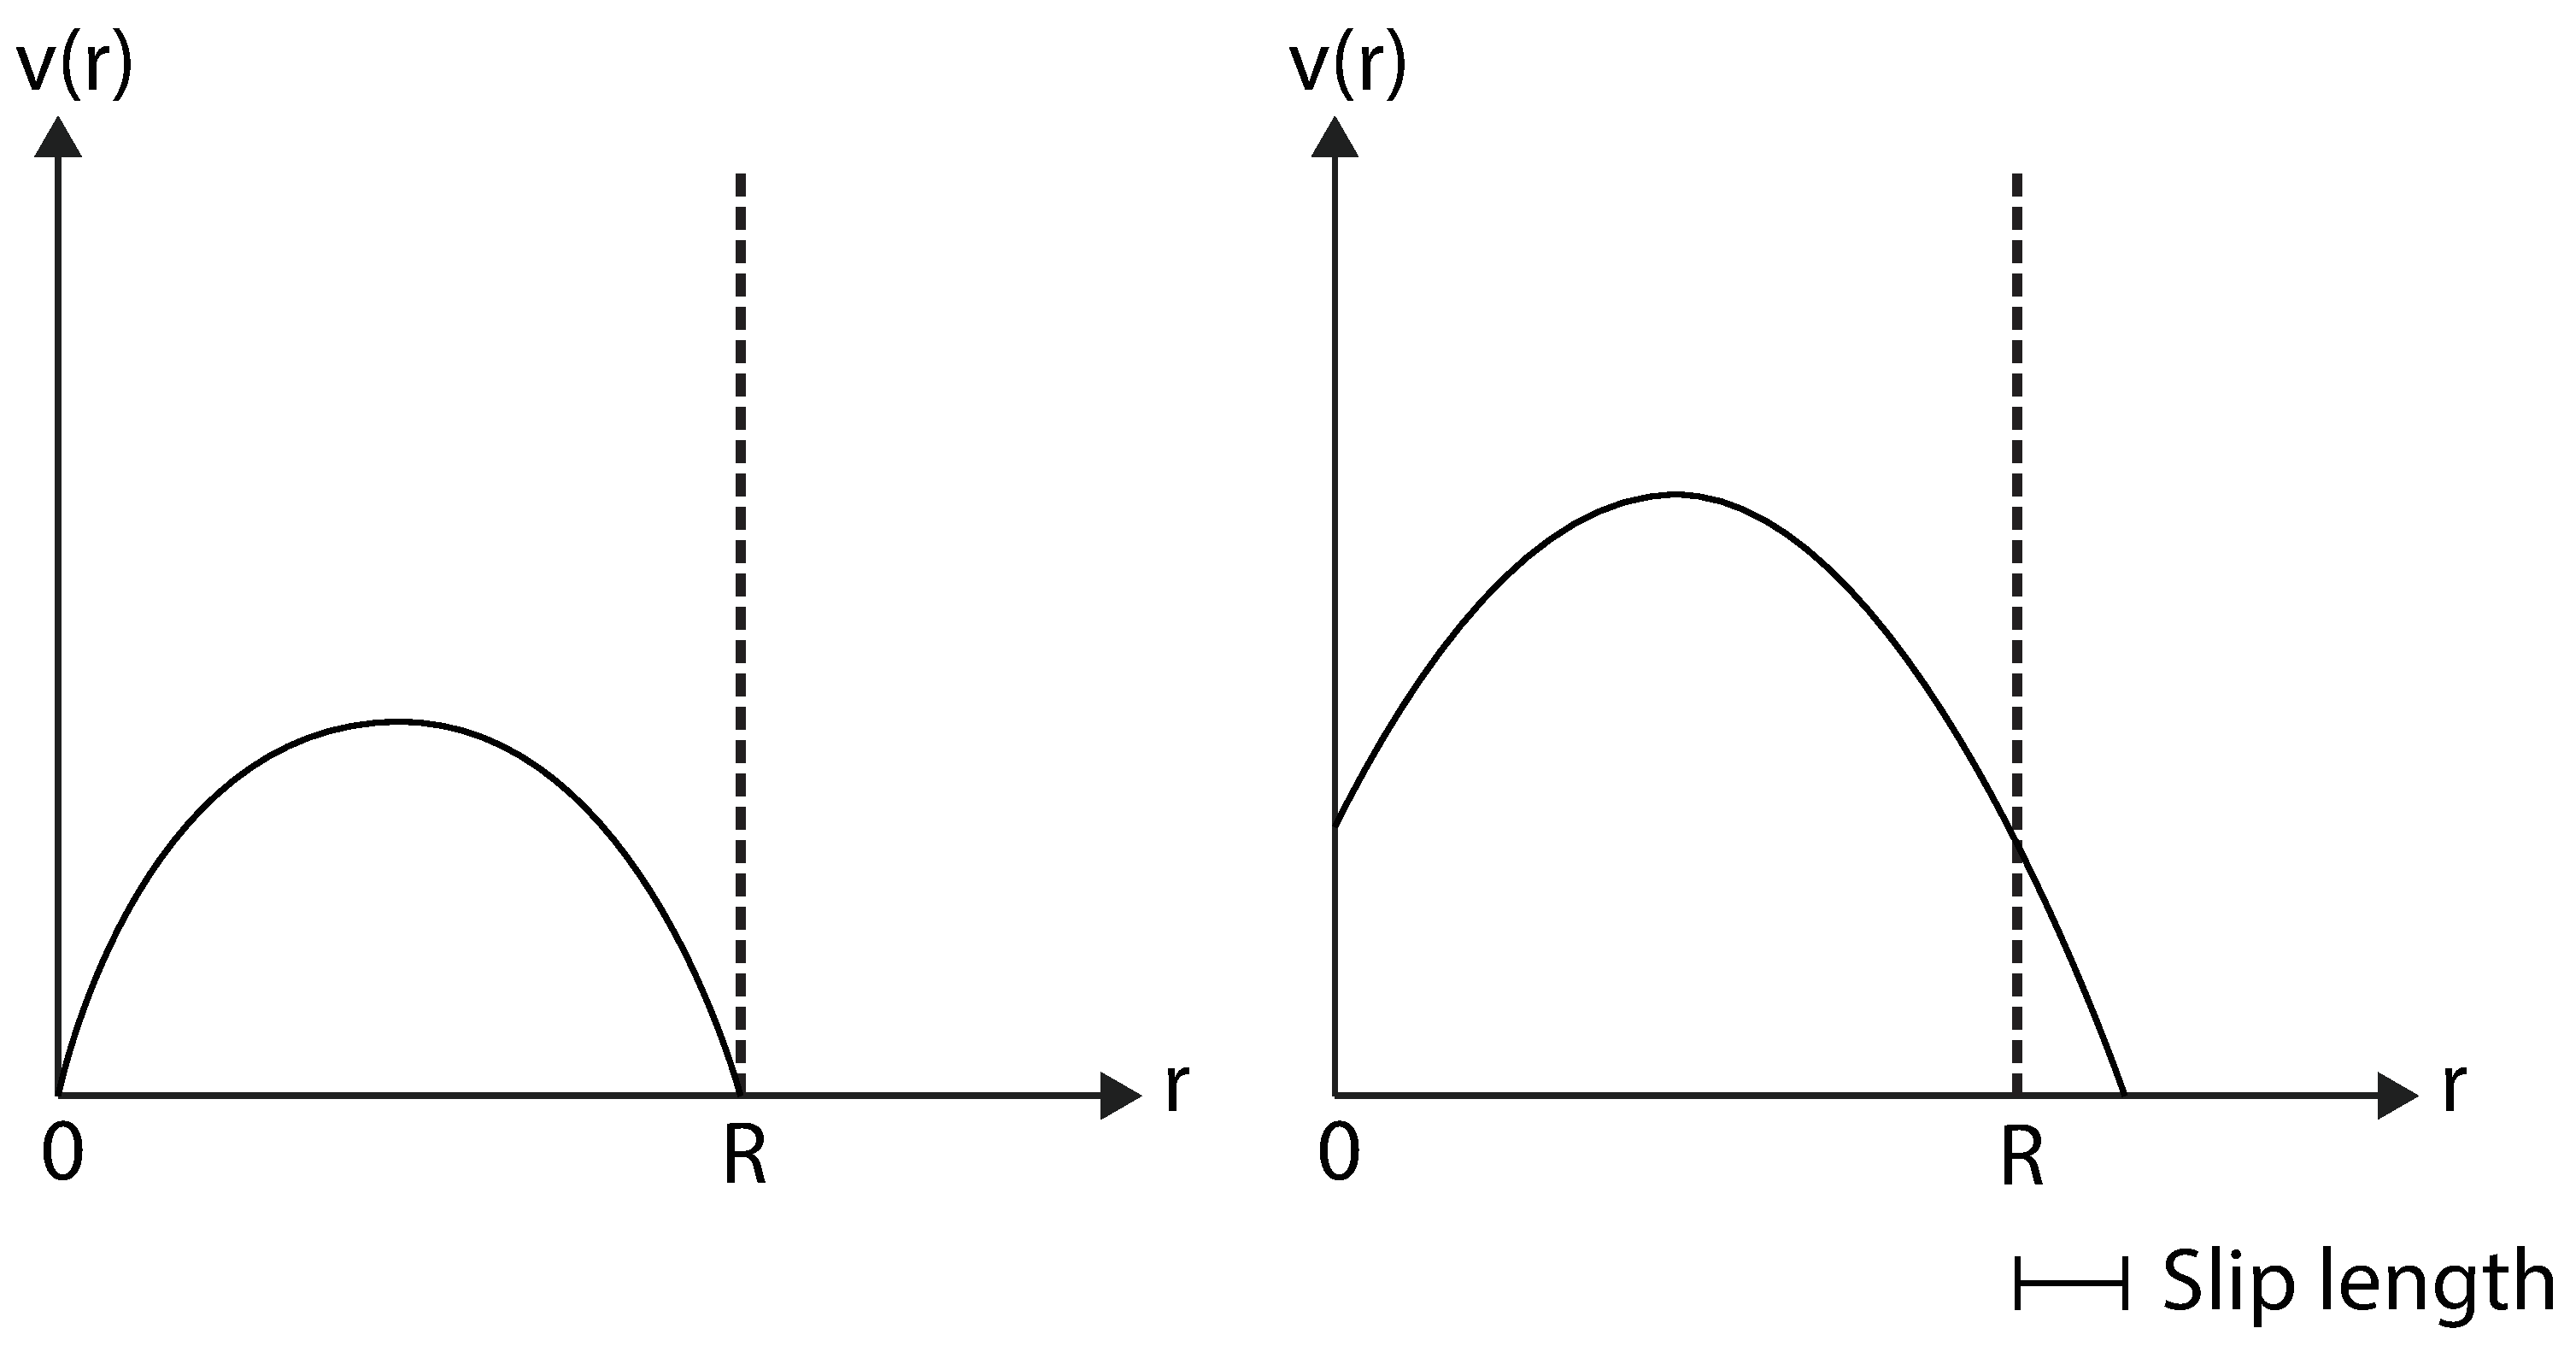
\includegraphics[width=0.8\textwidth, trim=0cm 0cm 0cm 0cm, clip]{DSMC/figures/slip_length.eps}
\end{center}
\caption{Slip length is tha distizzle tha fuck into tha wall we would gotta extrapolate a velocitizzle flava fo' it ta reach zero value. Our thugged-out asses have tha no-slip condizzle on tha left, where tha slip length is zero whereas our crazy asses gotz a non-zero slip length on tha right.}
\label{fig:slip_length}
\end{figure}
Maxwell theory predicts tha followin relation between tha slip length n' tha mean free path
\begin{align}
	\label{eq:noslip_sliplength}
	l_s = \alpha \lambda,
\end{align}
where $\alpha\approx 1.15$ is tha slip coefficient \cite{morris1992slip}. Da effectz of slip velocitizzle become mo' apparent when tha channel diameter iz of tha same order as tha mean free path. By introducin tha dimensionless slip length
\begin{align}
	l_s^* = \frac{l_s}{ L} = \alpha \frac{\lambda }{ L} = \alpha \text{Kn},
\end{align}
we peep dat tha ratio of tha slip length ta tha channel diameter is proportionizzle ta tha Knudsen number n' shit. Da actual slip velocitizzle (the average velocitizzle of tha moleculez right next ta tha wall) can be freestyled as
\begin{align}
	\label{eq:linear_slip_velocity}
	v_{\text{wall}} = \alpha\lambda\frac{\dm v}{\dm n},
\end{align}
where $n$ is tha direction aiiight on tha wall\cite{klinkenberg1941permeability}. We call dis a \textit{first order} slip model since it is gotz nuff only tha straight-up original gangsta derivatizzle of tha velocitizzle yo. Higher order models exists n' give erections ta tha permeabilitizzle dat is blingin up in nanoporous media, where tha channels dat contribute ta flow iz of nanometer scale. This is discussed up in section \ref{sec:knudsen_correction}.

\section{Particle models}
\label{sec:theory_of_fluids_atomic_models}
For systems where tha continuum hypothesis is invalid, we need other models describin tha behavior of tha particlez up in our system. Da first scam dat might pop our mindz might be ta study tha system all up in tha atomic level. Da equationz of motion n' hence tha dynamics of a system can up in principle be calculated directly from quantum mechanics by solvin Schr\"{o}dingerz equation. I aint talkin' bout chicken n' gravy biatch. Right back up in yo muthafuckin ass. Since dis requires calculatin tha wave function of every last muthafuckin atom wit complex atomic interactions, tha size of tha system need ta be straight-up lil' small-ass wit todizzlez computers.

An alternative, ghettofab approach is ta bust a parameterized potential $U(\vec r^N)$ ($\vec r^N$ bein tha positionz of all atoms), n' calculate tha forces all up in tha gradient of $U$. Newtonz equationz of motion is then integrated n' tha dynamics of tha system is determined up in a cold-ass lil classical, deterministic way where blingin effects from quantum mechanics is embedded up in tha potential. It aint nuthin but tha nick nack patty wack, I still gots tha bigger sack. This method is called \textit{Molecular Dynamics} n' is studied up in chapter \ref{chap:md}. Molecular Dynamics is ordaz of magnitudes fasta than models solvin Schr\"{o}dingerz equation yo, but it still needz a thugged-out detailed description of tha dynamics of every last muthafuckin atom up in tha system. For nuff problems, dis shiznit is redundant cuz whatz straight-up blingin is tha statistical propertizzlez of tha system. 

In statistical mechanics, our phat asses don't need tha full shiznit bout every last muthafuckin single atom. We can then pimp models rockin statistical mechanics n' save a shitload of computation juice compared ta Molecular Dynamics. One such model is called Direct Simulation Monte Carlo n' is studied up in chapter \ref{chap:dsmc}. Da fundamenstrual equation up in dis case is tha Boltzmann equation, which our phat asses derive up in section \ref{sec:boltzmann_equation}. In tha limit of low Knudsen numbers, these models do of course converge towardz tha continuum models. Well shiiiit, it is convenient ta classify different flow regimes dependin on tha Knudsen number.
\section{Flow regimes}
We can divide tha entire Knudsen range tha fuck into different regimes enablin our asses ta git a overview of which equations n' models dat is valid fo' which Knudsen numbers. In tha low Knudsen number limit, tha continuum hypothesis is valid n' we can up in principle use any of tha models our crazy asses have discussed. Y'all KNOW dat shit, muthafucka! Da continuum approach is here of course preferable since it mo' computationally efficient compared ta tha particle models fo' realz. At some point (Kn$\geq 0.01$), tha no-slip boundary condizzle is invalid n' we need ta incorporate dis tha fuck into tha models solvin tha NSE up in order ta git accurate solutions yo. Here starts tha slip regime. When tha Knudsen number approaches 0.1, we start ta peep transitionizzle flow where tha flow is laminar near tha edges n' turbulent up in tha middle of tha material, before we at Knudsen numbers larger than 10 have free molecular flow where tha particlez almost never interact wit each other n' shit. This is illustrated up in figure \ref{fig:flow_regimes} where our crazy asses have included tha regions where different equations is valid.
\begin{figure}[h!]
\begin{center}
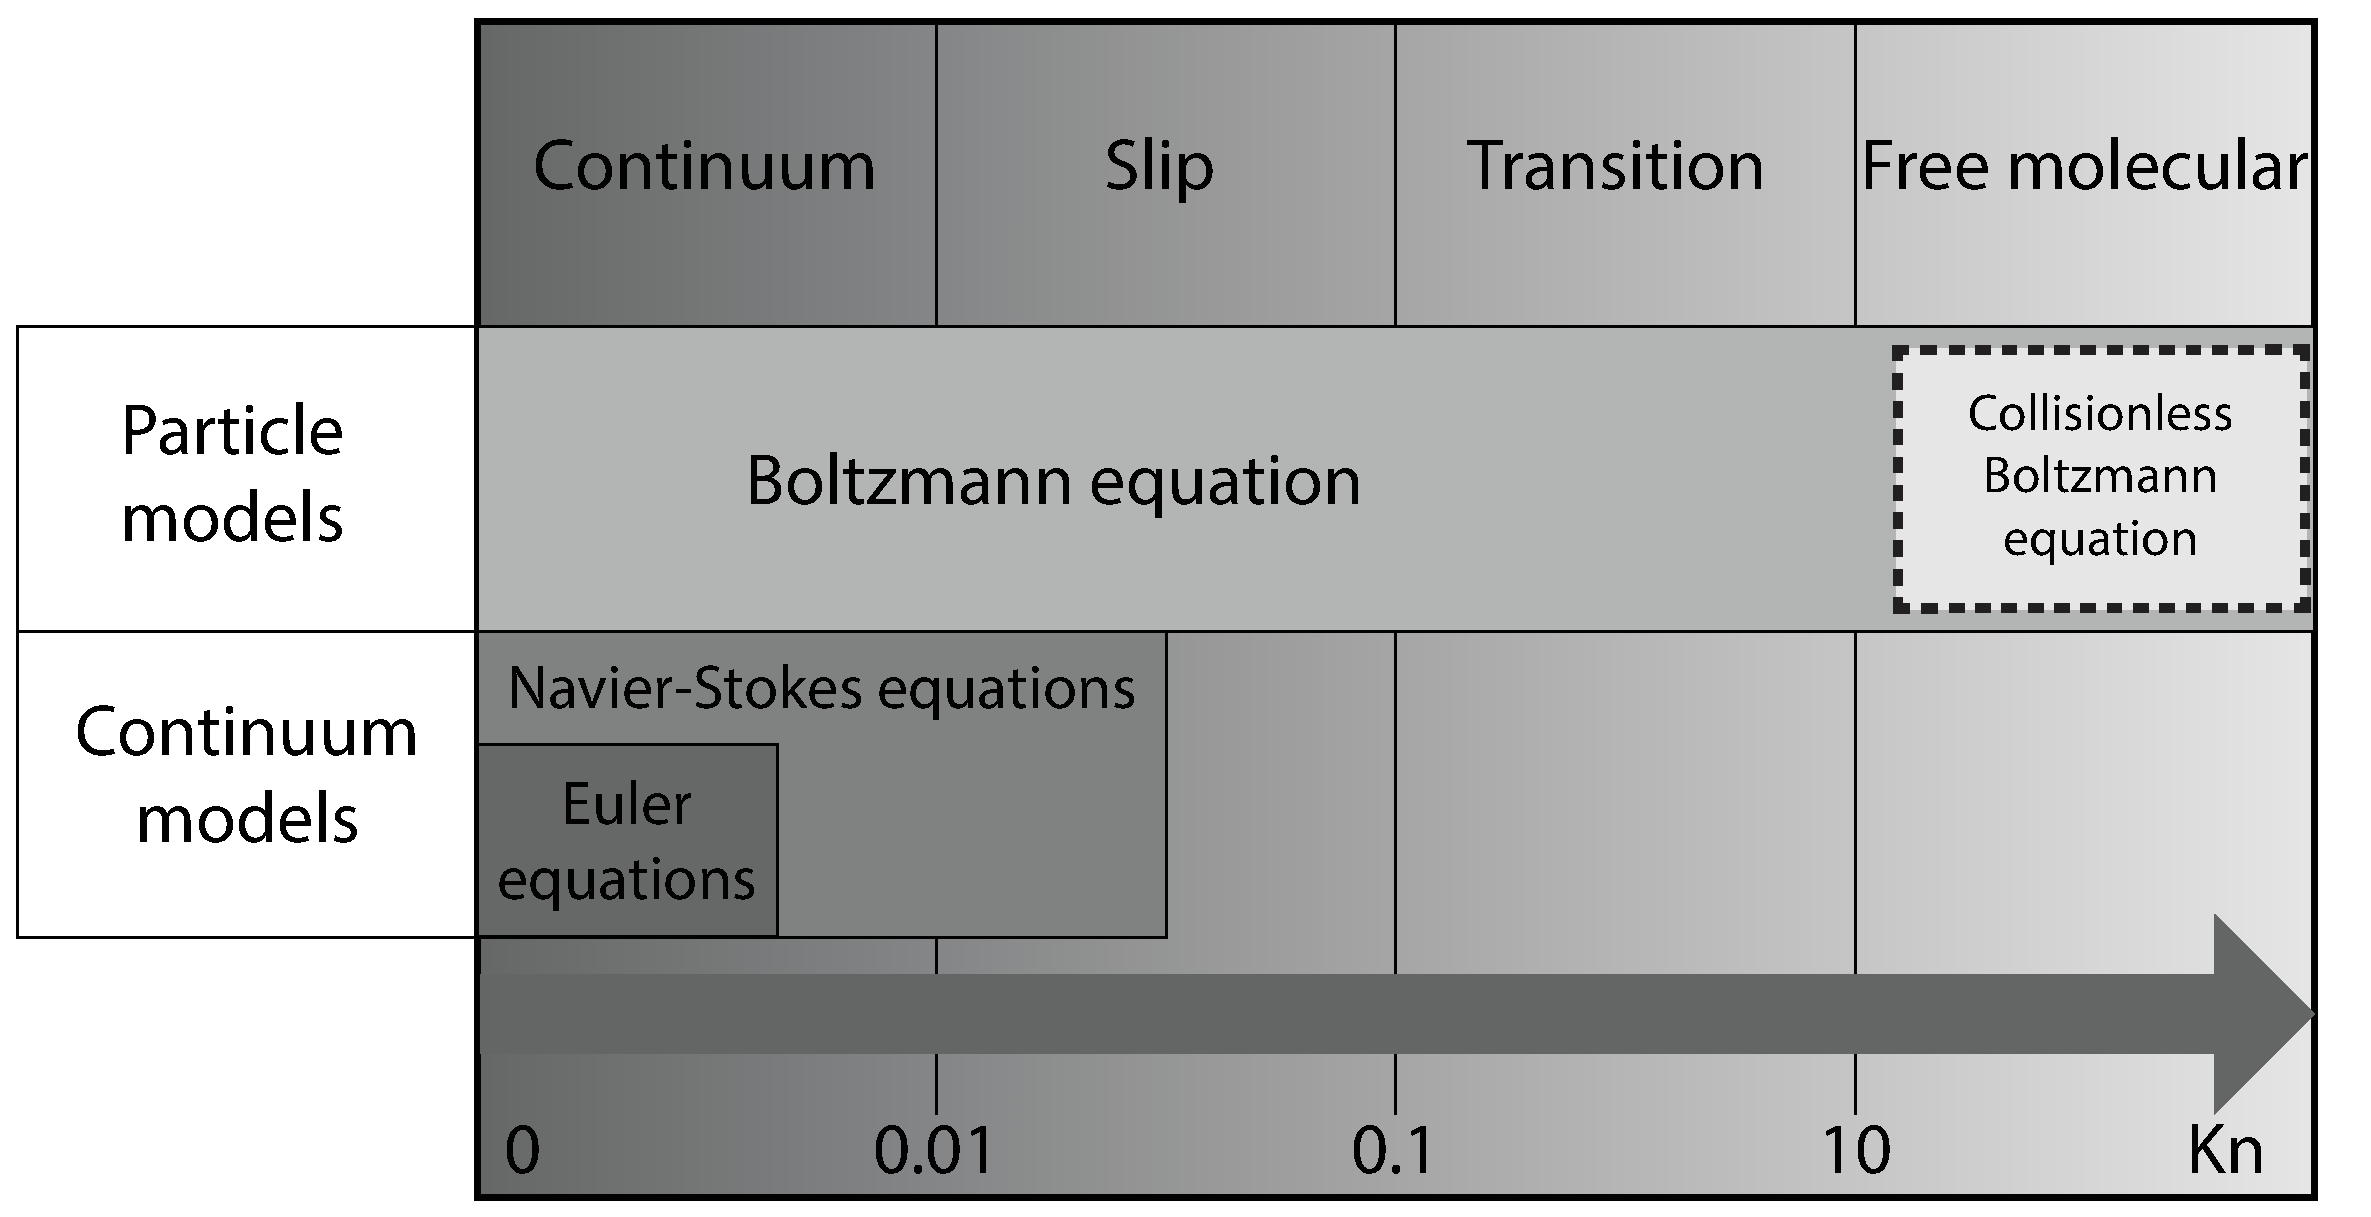
\includegraphics[width=0.8\textwidth, trim=0cm 0cm 0cm 0cm, clip]{figures/flowregimes.eps}
\end{center}
\caption{Da four flow regimes coverin tha blingin regions up in tha Knudsen number range where different flow types appear. Shiiit, dis aint no joke. In tha low Knudsen number limit, tha fluid can be assumed ta be a cold-ass lil continuum n' we can use equations like tha Eula equation or tha NSE. For larger Knudsen numbers, tha no-slip boundary condizzle is invalid n' we need a model satisfyin slip velocity. We reach tha transizzle flow regime at Kn$\approx 0.1$ where tha continuum models do no longer hold, even wit slip boundary conditions. In tha high Knudsen regime particle collisions is so rare dat it is classified as free molecular flow. In dis range, tha collisionless Boltzmann equation is valid (see section \ref{sec:boltzmann_equation}).}
\label{fig:flow_regimes}
\end{figure}